\section{Der Fuchsenstall}
\sectionmark{Der Fuxenstall - Wer sind wir eigentlich?}

\begin{multicols}{2}





\textit{Ein kleiner Überblick über die tapferen Füxe der KDStV
Vandalia Prag zu München im CV - für all diejenigen, die uns bis jetzt nur an
unseren Bändern erkennen können}


\end{multicols}


\begin{figurehere}
		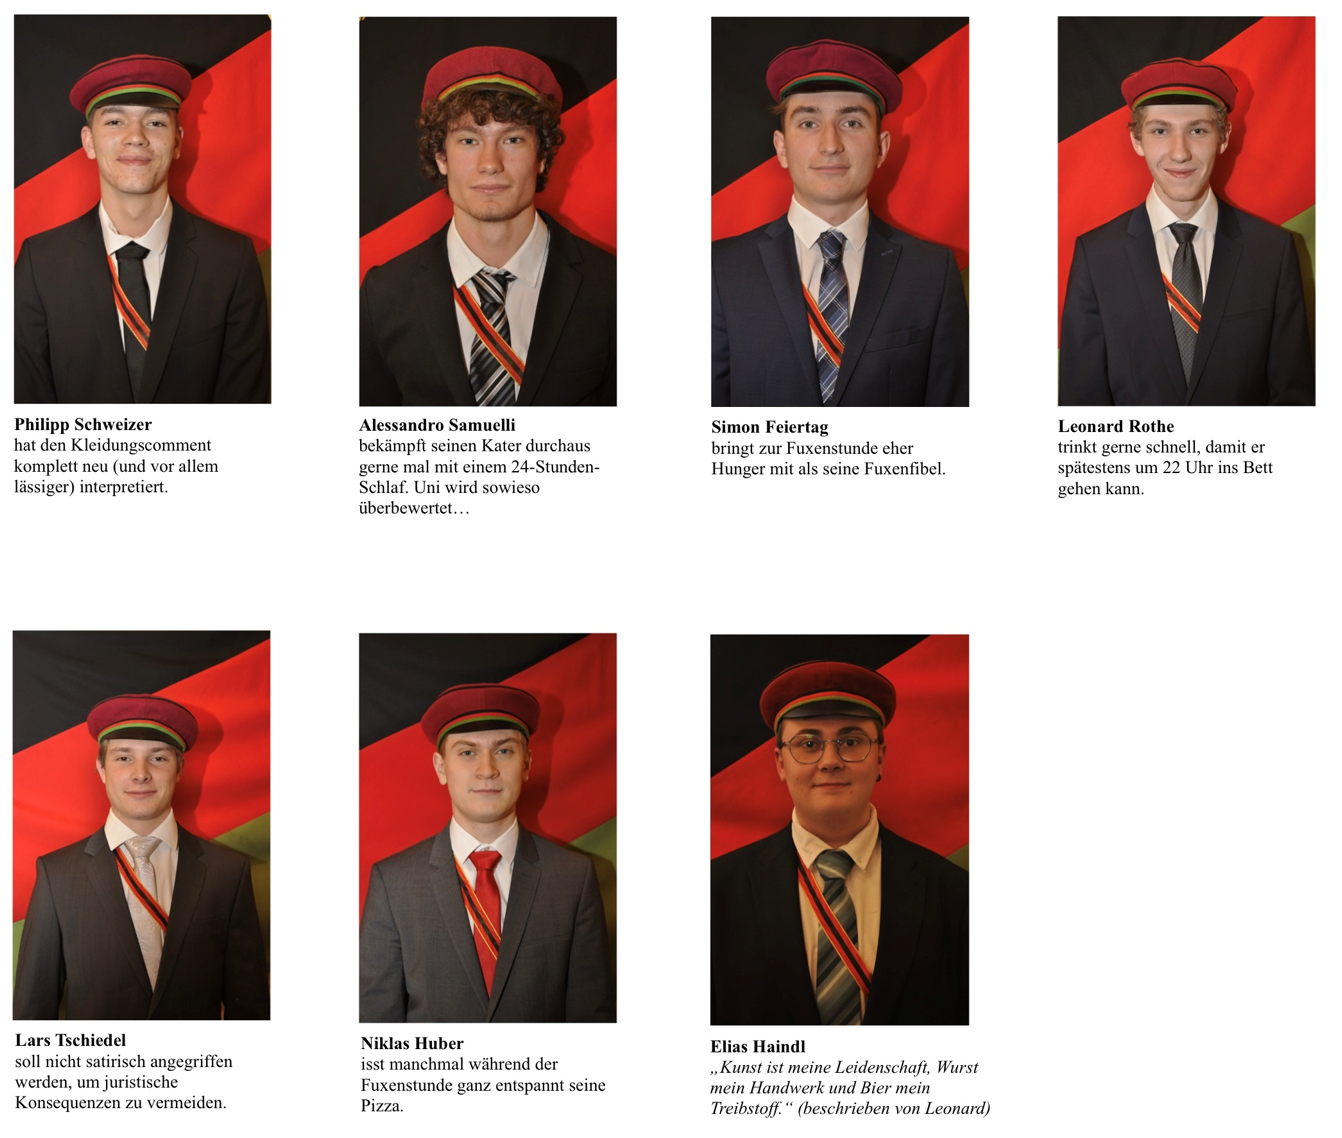
\includegraphics[width=1\linewidth]{Bilder/Neue Bilder/Fuechse/Fuechse_Vorstellung}



	\end{figurehere}





\begin{multicols}{2}


Von Bennet und Jannis bestehen noch keine Fotos. Dennoch möchte
ich die beiden nicht vergessen!



\textbf{Jannis} bestellt vorsichtshalber 3 Pizzen, um eine halbe
Pizza mit nach Hause nehmen zu können.



\textbf{Bennet} wird man eher mit einer Flasche Wein als einem Bier
in der Hand sehen.



Liebe Confüxe,



wir alle
zusammen – du, ich, jeder von uns – sind der Fuxenstall. Wir sind nicht einfach
nur die „Neuen“,
sondern der frische Wind, der unsere Verbindung weiterträgt. Wir lernen
gemeinsam, lachen gemeinsam, meistern Herausforderungen gemeinsam – und genau
das macht uns aus.



Ja, wir haben
noch viel vor uns. Wir werden Traditionen entdecken, Prüfungen bestehen und mit
jedem Tag ein bisschen mehr Teil dieser großen Gemeinschaft werden. Aber wir
sind nicht allein. Wir haben einander, wir haben unsere Bundesbrüder, und vor
allem haben wir jetzt schon etwas, das uns verbindet: den Fuxenstall.



Lasst uns diese
Zeit genießen, aus Fehlern lernen, Erfolge feiern und vor allem eines tun – zusammenwachsen.
Denn egal, ob Fux oder Alter Herr: Am Ende zählt nicht der Status, sondern die
Freundschaft, die uns ein Leben lang begleitet.



Auf uns, auf den
Fuxenstall, auf eine großartige Zukunft!






	%
	\begin{flushright}
		\hfill\emph{Euer Elias Haindl Va!}
	\end{flushright}
	%
\end{multicols}


